\documentclass[conference]{IEEEtran}
\IEEEoverridecommandlockouts
\usepackage[T1]{fontenc}
\usepackage[utf8]{inputenc}
\usepackage{cite}
\usepackage{amsmath,amssymb,amsfonts}
\usepackage{graphicx}
\usepackage{textcomp}
\usepackage{xcolor}
\usepackage{booktabs}
\usepackage{url}

\begin{document}

\title{Deep Learning-Based SNR Estimation from I/Q Samples: A Comparison with the M2M4 Estimator under Short Frames and Phase Impairments}

\author{\IEEEauthorblockN{Rıfat Burak Özkan}
\IEEEauthorblockA{\textit{Dept. of Electrical-Electronics Eng.} \\
\textit{Bursa Uludağ University}\\
Bursa, Türkiye \\
email address or ORCID}
\and
\IEEEauthorblockN{Arif Başgümüş}
\IEEEauthorblockA{\textit{Dept. of Electrical-Electronics Eng.} \\
\textit{Bursa Uludağ University}\\
Bursa, Türkiye \\
email address or ORCID}
\and
\IEEEauthorblockN{Murat Uyar}
\IEEEauthorblockA{\textit{Dept. of Electrical-Electronics Eng.} \\
\textit{Bursa Uludağ University}\\
Bursa, Türkiye \\
email address or ORCID}
}

\maketitle

\begin{abstract}
Accurate signal-to-noise ratio (SNR) estimation is required by receiver functions such as adaptive modulation, power control and link management. The moment-based M2M4 estimator is widely used because it is simple and does not require knowledge of the transmitted symbols, but its accuracy degrades severely at low SNR and with short observation windows. This paper compares M2M4 with learning-based estimators that predict the SNR directly from received QPSK in-phase and quadrature samples: a lightweight multilayer perceptron operating on moment-based features, a multilayer perceptron operating on raw samples, and a one-dimensional convolutional neural network. All models are trained and evaluated on simulated frames over an additive white Gaussian noise channel between minus 10 and 20 dB. For 1024-sample frames at or below minus 4 dB, the root mean square error of M2M4 is 11.4 dB, while the feature-based network and the convolutional network reduce it to 2.6 dB and 2.8 dB. With 128-sample frames, the overall error of M2M4 rises to 7.6 dB, whereas the feature-based network remains at 2.1 dB. Under phase and frequency offsets, networks trained only on clean data degrade markedly, while networks trained with these impairments retain their accuracy. The feature-based network, with about 4.8 thousand parameters, is the most accurate model in every experiment.
\end{abstract}

\begin{IEEEkeywords}
SNR estimation, deep learning, M2M4, convolutional neural network, QPSK, robustness
\end{IEEEkeywords}

\section{Introduction}

The signal-to-noise ratio (SNR) is one of the most frequently used measures of link quality in a digital receiver. Adaptive modulation and coding selects the constellation and code rate from the estimated SNR \cite{goldsmith1997}, power control uses it to adjust the transmit power, and soft-decision decoders use it to scale their reliability metrics. An SNR estimate that is biased or noisy therefore propagates into several receiver decisions.

Classical SNR estimators are commonly divided into data-aided estimators, which require known pilot symbols, and non-data-aided (blind) estimators, which operate on the received samples alone. Among the blind estimators, the second- and fourth-order moment estimator (M2M4) \cite{matzner1993} is attractive because it requires no symbol decisions, no carrier phase recovery and only a few arithmetic operations per sample. The comparative study in \cite{pauluzzi2000} shows, however, that the accuracy of moment-based estimators depends strongly on the SNR and on the number of available samples.

Deep learning has been applied increasingly to physical-layer problems \cite{oshea2017}, including modulation classification from raw in-phase and quadrature (I/Q) samples \cite{oshea2018}. Several recent studies have applied convolutional neural networks (CNNs) to SNR estimation, using input representations such as spectrograms of the I/Q components \cite{kojima2021}, power spectra and raw I/Q data \cite{zheng2024}, and a range of CNN architectures formulated as regression models \cite{mahbub2025}.

This paper presents a controlled comparison between M2M4 and three learning-based estimators of increasing input dimensionality: a small multilayer perceptron (MLP) operating on eight moment-based features, an MLP operating on raw I/Q samples, and a one-dimensional CNN. The contributions are as follows:
\begin{itemize}
\item a quantitative comparison under identical simulated data, splits and metrics, showing that learning-based estimators reduce the low-SNR error of M2M4 by a factor of about four;
\item an analysis of the effect of the frame length, showing that the advantage of the learned estimators increases as fewer samples are available;
\item a robustness analysis under carrier phase and frequency offsets, showing that models trained only on clean data degrade substantially and that training with these impairments removes most of the degradation;
\item the observation that a feature-based network with about 4.8 thousand parameters outperforms a CNN with about 81 thousand parameters in every experiment.
\end{itemize}

\section{System Model and Classical Estimator}

\subsection{Signal Model}

Each frame consists of $N$ complex baseband samples
\begin{equation}
r[k] = s[k] + w[k], \qquad k = 0, \ldots, N-1,
\label{eq:model}
\end{equation}
where $w[k]$ is circularly symmetric complex Gaussian noise with variance $\sigma^2$, and $s[k]$ is a QPSK symbol with unit average power, drawn uniformly from
\begin{equation}
s[k] \in \frac{1}{\sqrt{2}}\,\{1+j,\; 1-j,\; -1+j,\; -1-j\}.
\label{eq:qpsk}
\end{equation} Since the signal power is unity, the SNR of a frame is
\begin{equation}
\mathrm{SNR} = \frac{1}{\sigma^2}, \qquad \sigma^2 = 10^{-\mathrm{SNR_{dB}}/10}.
\label{eq:snr}
\end{equation}
Fig.~\ref{fig:const} shows received samples at four SNR values. At 20 dB the four clusters are clearly separated; at $-5$ dB they merge into a single cloud and the symbol from which a sample originated can no longer be inferred.

\begin{figure*}[!t]
\centering
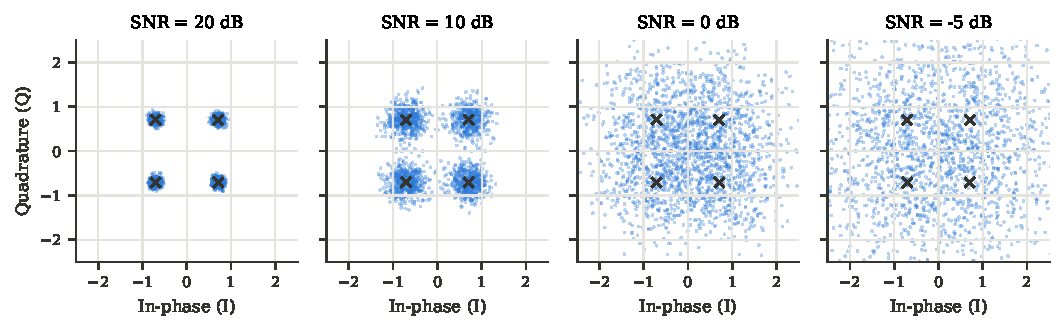
\includegraphics[width=\textwidth]{fig_constellation}
\caption{Received QPSK samples at different SNR values. Crosses mark the noise-free constellation points.}
\label{fig:const}
\end{figure*}

\subsection{M2M4 Estimator}

Let $M_2$ and $M_4$ denote the sample second- and fourth-order moments of the received frame,
\begin{equation}
M_2 = \frac{1}{N}\sum_{k=0}^{N-1} |r[k]|^2, \qquad M_4 = \frac{1}{N}\sum_{k=0}^{N-1} |r[k]|^4.
\label{eq:moments}
\end{equation}
For a constant-modulus constellation such as QPSK in complex Gaussian noise, the signal power $S$ and noise power $W$ satisfy $\mathrm{E}[M_2] = S + W$ and $\mathrm{E}[M_4] = S^2 + 4SW + 2W^2$. Solving for $S$ and $W$ gives the M2M4 estimates \cite{matzner1993, pauluzzi2000}
\begin{equation}
\hat{S} = \sqrt{2M_2^2 - M_4}, \qquad \hat{W} = M_2 - \hat{S},
\label{eq:m2m4}
\end{equation}
and the SNR estimate in decibels is
\begin{equation}
\widehat{\mathrm{SNR}}_{\mathrm{dB}} = 10\log_{10}\!\left(\hat{S}/\hat{W}\right).
\label{eq:snrhat}
\end{equation}
The estimator uses only the sample magnitudes and is therefore invariant to any phase rotation of the received frame. When the sample moments deviate from their expectations, $2M_2^2 - M_4$ or $\hat{W}$ can become negative; such frames are counted as invalid, and their estimates are clipped to the interval $[-30, 50]$ dB so that the error remains finite.

\section{Learning-Based Estimators}

\subsection{Input Normalization}

Before being passed to a network, every frame is scaled to unit average power, which corresponds to the automatic gain control of a practical receiver. Without this step a network could infer the SNR from the total received power $1 + \sigma^2$, which is not available to a real receiver whose signal power is unknown. M2M4 is unaffected by this scaling.

\subsection{Feature-Based MLP}

Eight scale-invariant features are extracted from each normalized frame: the moment ratios $M_4/M_2^2$ and $M_6/M_2^3$; the standard deviations of $|r[k]|$ and $|r[k]|^2$; the mean absolute values of the in-phase and quadrature components; the fourth-order statistic
\begin{equation}
C_4 = -\mathrm{Re}\Big\{\frac{1}{N}\sum_{k=0}^{N-1} r^4[k]\Big\},
\label{eq:c4}
\end{equation}
which equals one for noise-free, phase-aligned QPSK; and the M2M4 estimate divided by ten. The features are standardized with the mean and standard deviation of the training set. The network has two hidden layers of 64 units with ReLU activations and a single linear output, for a total of 4\,801 parameters.

\subsection{Raw-Sample MLP}

The raw-sample MLP receives the $2N$ real values of the normalized frame and has hidden layers of 512, 256 and 64 units with ReLU activations and a dropout rate of 0.2.

\subsection{One-Dimensional CNN}

The CNN receives the frame as a two-channel sequence (I and Q) of length $N$. It contains three convolutional blocks with 32, 64 and 128 filters of length 7, each followed by batch normalization \cite{ioffe2015}, a ReLU activation and max pooling by a factor of two. Global average pooling, a 64-unit fully connected layer with dropout of 0.2 and a linear output follow. Global average pooling makes the network independent of the frame length. The model has 81\,121 parameters.

\subsection{Training}

All networks regress the SNR in decibels and are trained with the mean squared error loss and the Adam optimizer \cite{kingma2015} with a batch size of 256. The learning rate is halved when the validation loss does not improve for three epochs, and training stops when the validation loss does not improve for a fixed number of epochs, after which the best weights are restored. The feature-based MLP uses an initial learning rate of $10^{-3}$, at most 50 epochs and a stopping patience of 8 epochs. The CNN uses an initial learning rate of $3 \times 10^{-4}$, at most 60 epochs and a patience of 12 epochs, which reduced the fluctuation of its validation loss observed in preliminary runs. The models are implemented in PyTorch \cite{paszke2019} and trained on an NVIDIA T4 GPU.

\section{Experimental Setup}

\begin{figure}[!t]
\centering
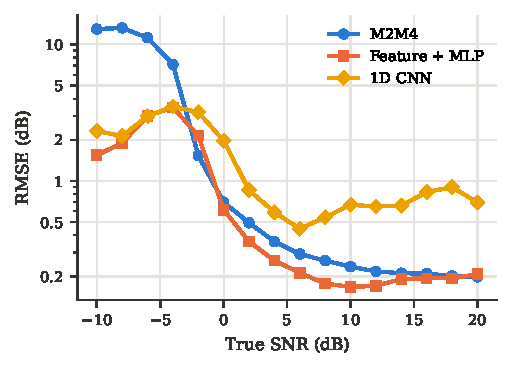
\includegraphics[width=\columnwidth]{fig_rmse_vs_snr}
\caption{RMSE versus true SNR for $N = 1024$ over AWGN.}
\label{fig:rmse}
\end{figure}

\begin{figure*}[!t]
\centering
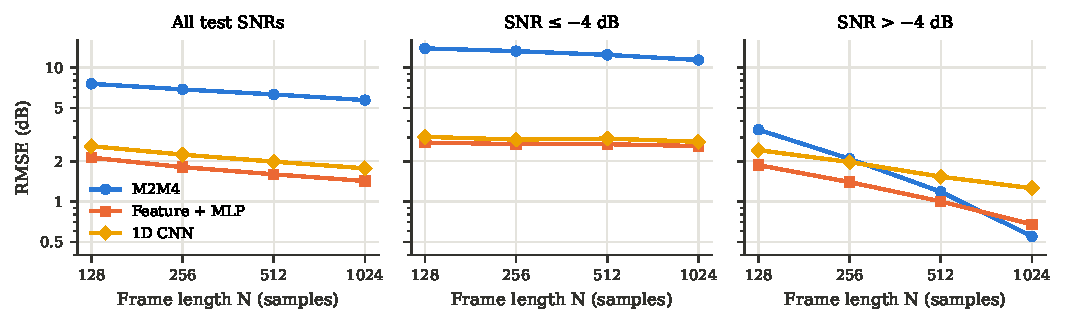
\includegraphics[width=\textwidth]{fig_frame_length}
\caption{RMSE versus frame length over AWGN: all test SNRs (left), SNR $\leq -4$ dB (centre) and SNR $> -4$ dB (right).}
\label{fig:framelen}
\end{figure*}


For each frame length, 50\,000 training frames and 10\,000 validation frames are generated with SNR values drawn uniformly from $[-15, 25]$ dB. The training range extends 5 dB beyond the test range on both sides to reduce the regression of the estimates toward the centre of the training distribution near the edges of the test range. The test set contains 1\,000 frames at each SNR from $-10$ to 20 dB in steps of 2 dB, that is, 16\,000 frames per frame length. Training, validation and test sets are generated with different random seeds.

The performance measure is the root mean square error (RMSE) between the estimated and true SNR in decibels. Results are reported over the whole test range and separately for SNR $\leq -4$ dB, the region in which M2M4 breaks down, and for SNR $> -4$ dB. The simulation, training and evaluation code is publicly available at \url{https://github.com/rftbrkzkn/snr-estimation-dl}.

\section{Results}

\subsection{Comparison over AWGN}\label{sec:awgn}

Table~\ref{tab:awgn} and Fig.~\ref{fig:rmse} summarize the results for $N = 1024$. Above $-4$ dB, M2M4 is accurate, with an RMSE of 0.55 dB that falls to about 0.2 dB at high SNR. Below this point it breaks down: the RMSE exceeds 11 dB between $-10$ and $-6$ dB, and 39\% of the frames at $-10$ dB produce invalid estimates. Both learned estimators remain usable throughout this region and reduce the low-SNR RMSE by a factor of about four. From 0 dB upward, the feature-based MLP matches or slightly improves on M2M4; its aggregate RMSE above $-4$ dB (0.68 dB) is nevertheless higher than that of M2M4 (0.55 dB), mainly because of the transition region around $-2$ dB. For SNR $\geq 2$ dB, the CNN retains a residual error of 0.45--0.9 dB.

\begin{table}[!t]
\caption{RMSE (dB) of the estimators over AWGN for $N = 1024$}
\label{tab:awgn}
\centering
\setlength{\tabcolsep}{4pt}
\begin{tabular}{@{}lrrrr@{}}
\toprule
 & & \multicolumn{3}{c}{RMSE (dB)} \\
\cmidrule(l){3-5}
Method & Params & All & $\leq -4$ dB & $> -4$ dB \\
\midrule
M2M4 & -- & 5.71 & 11.38 & \textbf{0.55} \\
Feature-based MLP & 4\,801 & \textbf{1.42} & \textbf{2.59} & 0.68 \\
1D CNN & 81\,121 & 1.77 & 2.79 & 1.26 \\
\bottomrule
\end{tabular}
\end{table}

The raw-sample MLP did not generalize. In a preliminary experiment with training and test SNRs both drawn from $[-10, 20]$ dB, its training error decreased while its validation error increased from the first epochs, and its predictions remained close to a constant value regardless of the true SNR, giving an overall RMSE of 9.36 dB. The SNR is encoded in the distribution of the sample magnitudes rather than in the position of individual samples within the frame. A fully connected network has to learn this permutation-invariant property from data, whereas the weight sharing and global pooling of the CNN, and the explicit moment features of the feature-based MLP, provide it by construction. The raw-sample MLP is therefore excluded from the remaining experiments.

At low SNR, both learned estimators show a negative bias of about 2.0--2.8 dB between $-6$ and $-4$ dB. In this region the frames carry little information about the SNR, and the regression estimate approaches the conditional mean of the training distribution. The bias thus depends on the SNR distribution used during training, which should be chosen to match the operating range of the target receiver.

\subsection{Effect of the Frame Length}

\begin{figure}[!t]
\centering
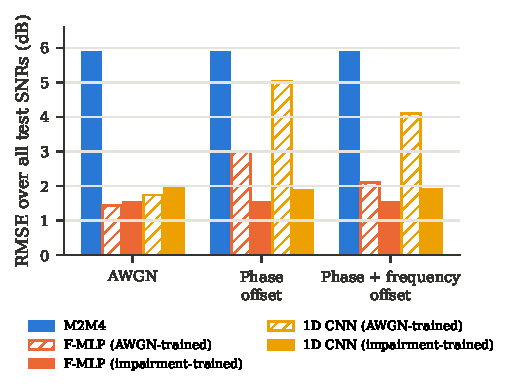
\includegraphics[width=\columnwidth]{fig_robustness}
\caption{RMSE over all test SNRs ($N = 1024$) for clean AWGN, a random phase offset, and a random phase and frequency offset. Hatched bars denote networks trained only on AWGN.}
\label{fig:robust}
\end{figure}


Fig.~\ref{fig:framelen} shows the RMSE as the frame length is reduced from 1\,024 to 128 samples. All estimators degrade with fewer samples, because the sample moments and learned statistics become less reliable, but M2M4 degrades most. Its overall RMSE increases from 5.71 to 7.56 dB, while that of the feature-based MLP increases from 1.42 to 2.13 dB. The difference is most visible above $-4$ dB: the RMSE of M2M4 increases from 0.55 dB at $N = 1024$ to 3.43 dB at $N = 128$, whereas the feature-based MLP reaches 1.87 dB at $N = 128$. For $N \leq 512$, the feature-based MLP is more accurate than M2M4 in both SNR regions, which is relevant for receivers that must estimate the SNR from short packets or rapidly varying channels.

\subsection{Robustness to Phase and Frequency Offsets}

Practical receivers estimate the SNR before carrier synchronization is complete. To assess robustness, test frames are rotated by a random phase $\theta$ drawn uniformly from $[0, 2\pi)$, and, in a second scenario, additionally subjected to a carrier frequency offset $f$ drawn uniformly from $[-0.005, 0.005]$ cycles per sample, so that each received sample becomes
\begin{equation}
\tilde{r}[k] = r[k]\, e^{\,j(\theta + 2\pi f k)}.
\label{eq:impair}
\end{equation} Two versions of each network are compared: one trained on AWGN only (Section~\ref{sec:awgn}) and one trained on frames with random phase and frequency offsets drawn from the same distributions.

Fig.~\ref{fig:robust} shows the results. As expected from \eqref{eq:m2m4}, M2M4 is unaffected because it depends only on $|r[k]|$. The networks trained only on AWGN degrade substantially: the RMSE of the CNN increases from 1.74 to 5.03 dB under a phase offset, and that of the feature-based MLP from 1.43 to 3.01 dB, because several of its features depend on the phase of the constellation. The degradation is smaller under the combined offset; a detailed analysis of this effect is left for future work. Training with the impairments removes most of this sensitivity: the feature-based MLP achieves 1.53 dB and the CNN 1.88--1.89 dB in both impaired scenarios, at the cost of a small increase in error on clean AWGN data (from 1.43 to 1.51 dB and from 1.74 to 1.94 dB, respectively). Learned SNR estimators should therefore be trained on data that reproduce the impairments expected at their position in the receiver chain.

\subsection{Complexity}

The feature-based MLP has about one seventeenth of the parameters of the CNN, and its input dimension does not depend on $N$. Its feature extraction requires a small number of operations per sample, comparable to those of M2M4, followed by a network with fewer than five thousand weights. Together with its accuracy, this makes it a suitable candidate for implementation in resource-constrained receivers.

\section{Conclusion}

This paper compared the classical M2M4 SNR estimator with three learning-based estimators on simulated QPSK frames. Learned estimators reduce the RMSE below $-4$ dB from 11.4 dB to 2.6--2.8 dB, and their advantage increases as the frame length decreases. Networks trained only on clean AWGN data are sensitive to phase and frequency offsets, whereas training with these impairments restores their accuracy. A feature-based MLP with 4\,801 parameters outperformed a 1D CNN with 81\,121 parameters in every experiment, while a fully connected network on raw samples failed to generalize. Future work will extend the evaluation to higher-order modulations, fading channels and over-the-air measurements with software-defined radios.

\section*{Acknowledgment}

The authors used Claude (Anthropic) to assist with the development of the simulation and training code, the preparation of the figures and the drafting of the manuscript text. All experiments were executed by the authors, and all results, analyses and text were reviewed, verified and edited by the authors, who take full responsibility for the content of this paper.

\begin{thebibliography}{00}
\bibitem{goldsmith1997} A. J. Goldsmith and S.-G. Chua, ``Variable-rate variable-power MQAM for fading channels,'' \textit{IEEE Trans. Commun.}, vol. 45, no. 10, pp. 1218--1230, Oct. 1997.
\bibitem{matzner1993} R. Matzner, ``An SNR estimation algorithm for complex baseband signals using higher order statistics,'' \textit{Facta Universitatis (Niš), Ser. Electron. Energ.}, vol. 6, no. 1, pp. 41--52, 1993.
\bibitem{pauluzzi2000} D. R. Pauluzzi and N. C. Beaulieu, ``A comparison of SNR estimation techniques for the AWGN channel,'' \textit{IEEE Trans. Commun.}, vol. 48, no. 10, pp. 1681--1691, Oct. 2000.
\bibitem{oshea2017} T. O'Shea and J. Hoydis, ``An introduction to deep learning for the physical layer,'' \textit{IEEE Trans. Cogn. Commun. Netw.}, vol. 3, no. 4, pp. 563--575, Dec. 2017.
\bibitem{oshea2018} T. J. O'Shea, T. Roy, and T. C. Clancy, ``Over-the-air deep learning based radio signal classification,'' \textit{IEEE J. Sel. Topics Signal Process.}, vol. 12, no. 1, pp. 168--179, Feb. 2018.
\bibitem{kojima2021} S. Kojima, Y. Feng, K. Maruta, K. Ootsu, T. Yokota, C.-J. Ahn, and V. Tarokh, ``Investigation of input signal representation to CNN for improving SNR classification accuracy,'' in \textit{Proc. IEEE 94th Veh. Technol. Conf. (VTC2021-Fall)}, 2021, doi: 10.1109/VTC2021-Fall52928.2021.9625566.
\bibitem{zheng2024} S. Zheng, S. Chen, T. Chen, Z. Yang, Z. Zhao, and X. Yang, ``Deep learning-based SNR estimation,'' \textit{IEEE Open J. Commun. Soc.}, vol. 5, pp. 4778--4796, 2024.
\bibitem{mahbub2025} A. Al Mahbub, I. Ahmad, and S. Shin, ``Comprehensive analysis of CNN-based models for SNR estimation,'' \textit{IEEE Access}, vol. 13, pp. 213346--213361, 2025.
\bibitem{ioffe2015} S. Ioffe and C. Szegedy, ``Batch normalization: Accelerating deep network training by reducing internal covariate shift,'' in \textit{Proc. 32nd Int. Conf. Mach. Learn. (ICML)}, 2015, pp. 448--456.
\bibitem{kingma2015} D. P. Kingma and J. Ba, ``Adam: A method for stochastic optimization,'' in \textit{Proc. 3rd Int. Conf. Learn. Represent. (ICLR)}, 2015.
\bibitem{paszke2019} A. Paszke \textit{et al.}, ``PyTorch: An imperative style, high-performance deep learning library,'' in \textit{Adv. Neural Inf. Process. Syst. (NeurIPS)}, vol. 32, 2019.
\end{thebibliography}

\end{document}
